% !TEX root = ../supp.tex
\begin{figure}[h!]
\centering
\iflatexml
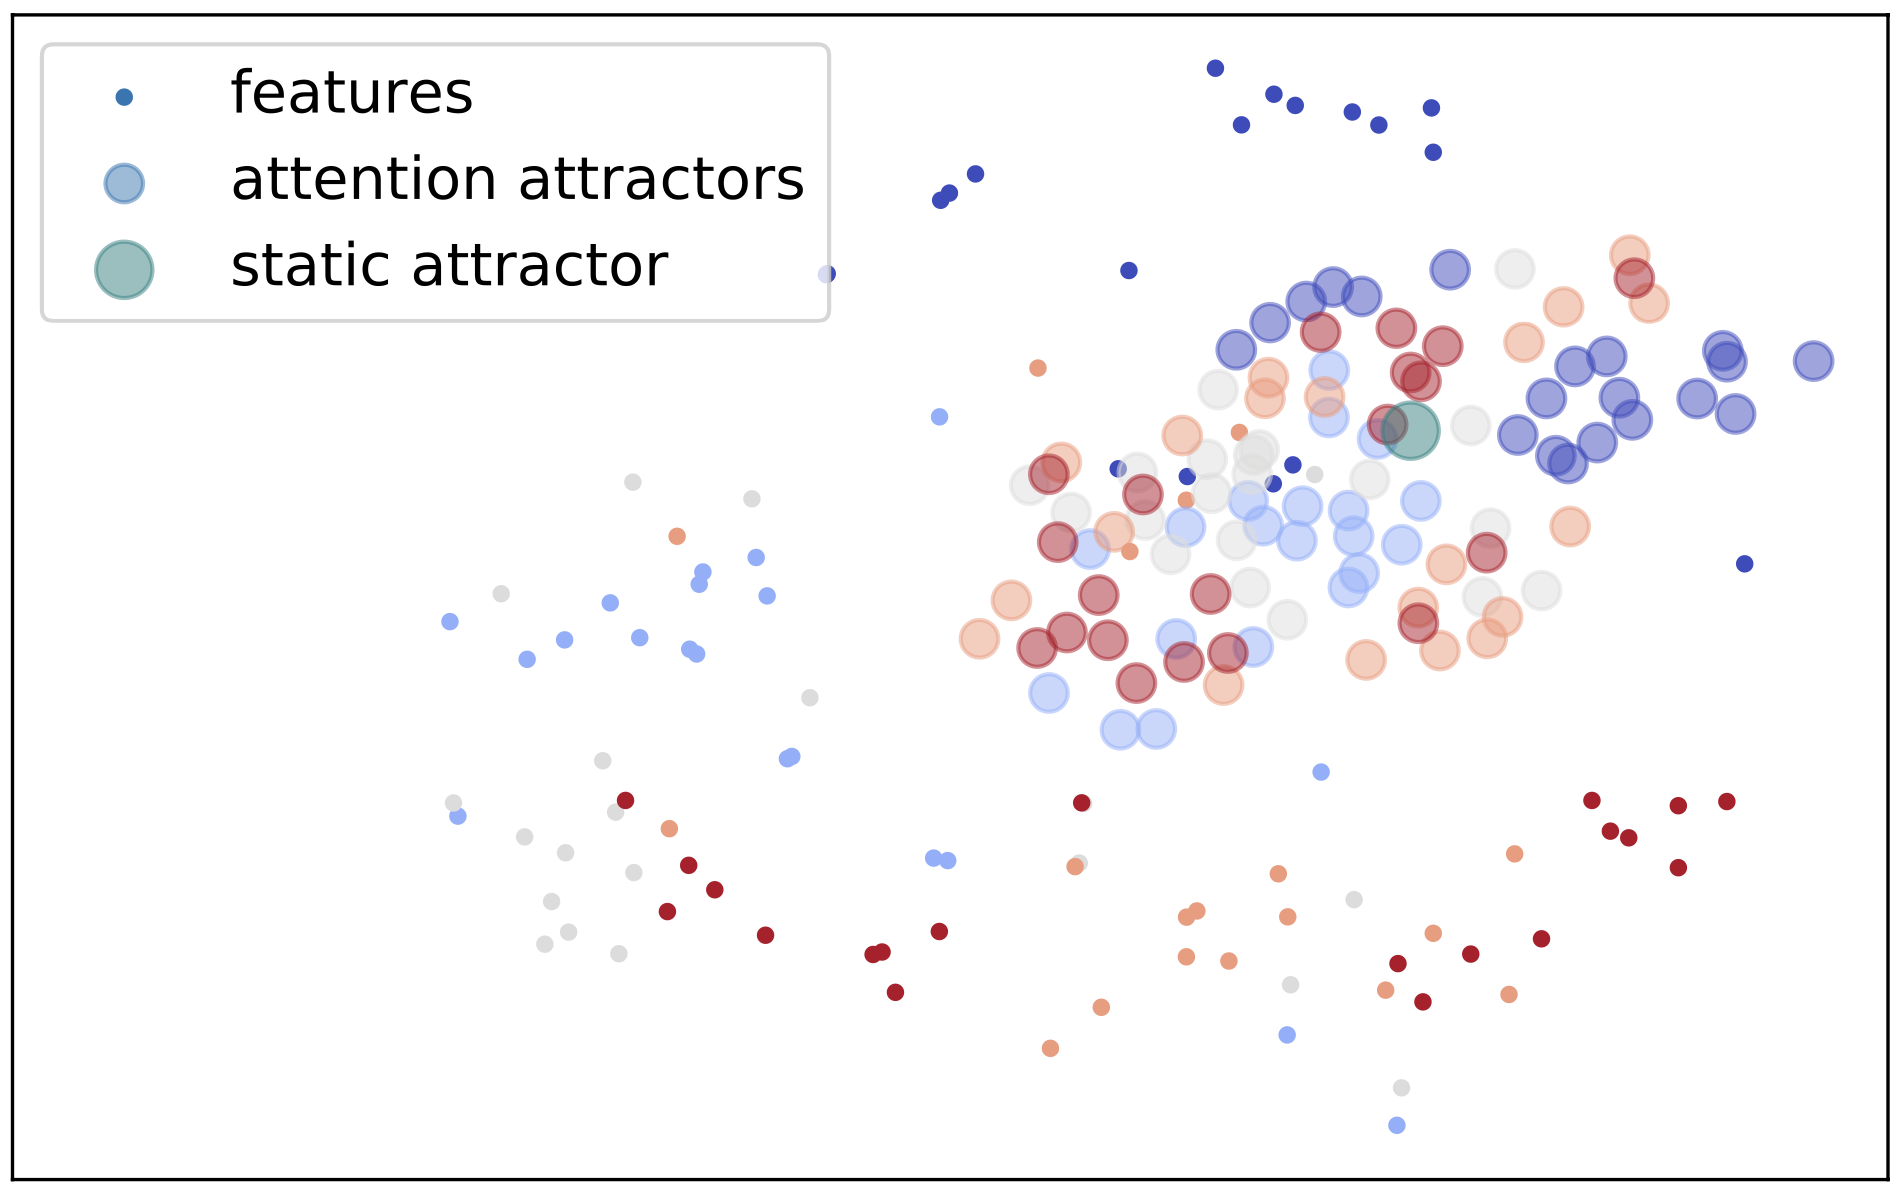
\includegraphics[width=4\textwidth]{figures/attractor_tsne.png}
\else
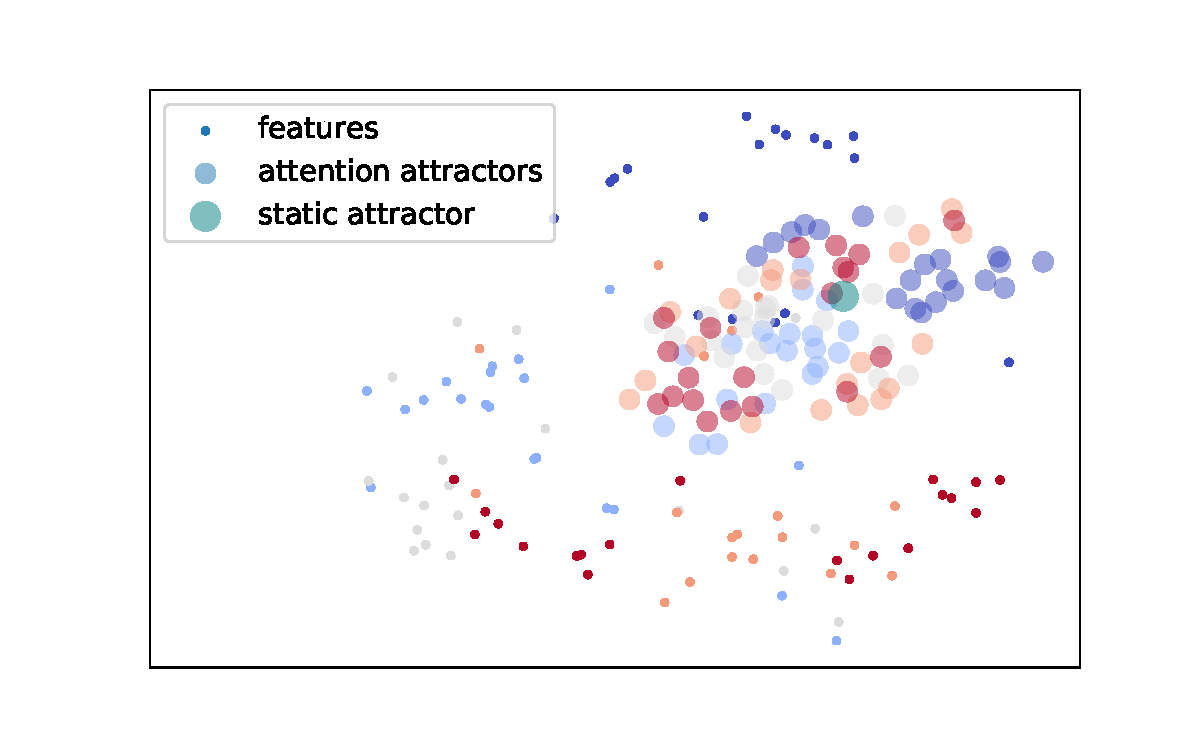
\includegraphics[width=0.6\textwidth,trim={1cm 0.5cm 1.6cm 1cm},clip]{figures/attractor_tsne.pdf}
\fi
\caption{Visualization of example features and attractors using t-SNE. This plot shows a 5-way
5-shot episode on \textit{mini}-ImageNet. 512-dimensional feature vectors and attractor vectors
are projected to a 2-dim space. Color represents the label class of the example. The static
attractor (\textcolor{teal}{teal}) appears at the center of the attention attractors, which roughly
form clusters based on the classes.}
\label{fig:attractorviz}
\end{figure}
